% !TeX spellcheck = da_DK
\subsection{Software}\label{software_test_implem}
Patienternes data skal behandles i form af grafisk visualisering, jævnfør afsnit \ref{subsec:software}, side \pageref{subsec:software}. Derudover skal patienternes resultater kunne gemmes til analyse og senere brug. For at imødekomme disse krav anvendes en computer med programmet MATLAB. Der designes en Graphical User Interface (GUI), hvor signalet fra accelerometeret visualiseres. MATLAB koden, der anvendes ved optagelse af signalet, er vedlagt i bilag \ref{Bilag:software}, side \pageref{Bilag:software}.\\ 
Signalet optages i MATLAB igennem den digitale del af systemet. Der designes en GUI for at optimere brugervenligheden for softwaren. I GUI'en ses en graf samt fire knapper og en toolbar, hvilket er illustretet på \figref{Fig:GUI_generisk}. 
\begin{figure}[H] 
	\centering 
	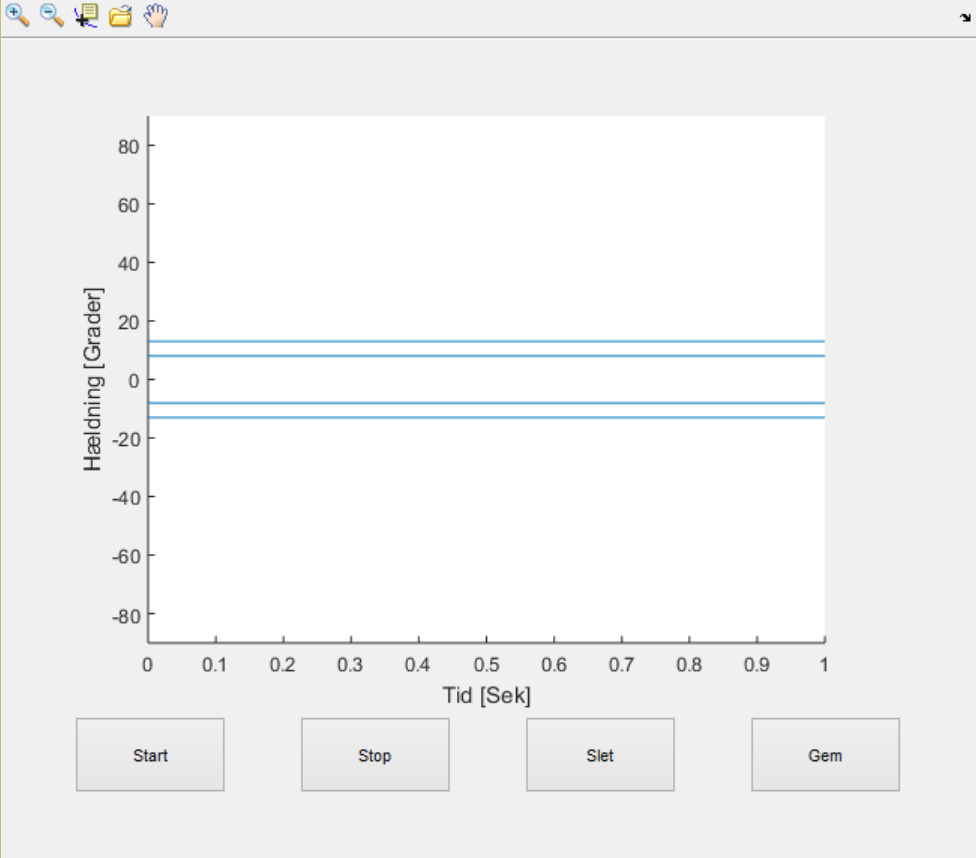
\includegraphics[scale=0.5]{figures/cProblemloesning/GUI_generisk.PNG}
	\caption{Af figuren fremgår GUI'ens display. De blå linjer illustrer de forskellige tærskelværdier i positiv og negativ retning for hhv. $\pm 8^{\circ}$ og $\pm 13^{\circ}$.}
	\label{Fig:GUI_generisk}
\end{figure} 
\noindent I koordinatsystemet er y-aksen hældningen i grader, mens x-aksen er tiden i sekunder. Dette skal gøre det enkelt for plejepersonalet at se, hvilken side patienten hælder til, samt i hvor lang tid patienten befinder sig i denne position. De fire blå linjer på tværs af koordinatsystemet er referencelinjer, der illustrerer de opstillede tærskelværdier i feedbackblokken. I displayet ses en start-, stop-, slette- og gemmefunktion.
I toolbaren er der flere knapper, som har hvert deres formål. Forstørrelsesglasset med plusset gør det muligt at zoome ind på grafen, mens forstørrelsesglasset med minusset gør det muligt at zoome ud igen. Knappen med et papir og et plus gør det muligt at aflæse det præcise punkt på grafen, der markeres. Mappen gør det muligt at åbne en fil i GUI'en, og hånden gør det muligt at navigere på displayet.\\
For at benytte GUI'en skal det fagkyndige personale følge fremgangsmåden, som fremgår på \figref{Fig:fremgangsmåde_software}.
\begin{figure}[H] 
	\centering 
	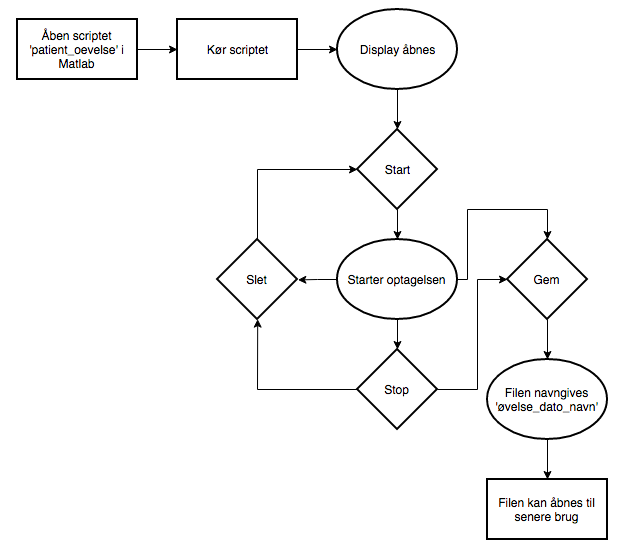
\includegraphics[scale=0.5]{figures/cProblemloesning/Software_flowdiagram.PNG}
	\caption{På figuren ses et flowdiagram over fremgangsmåden for personalet til at benytte softwaren.}
	\label{Fig:fremgangsmåde_software}
\end{figure}

\subsubsection{Test}
For at teste hvorvidt softwaren viser den forventede information omkring patientens kropshældning, indsendes et input så tæt på det teoretiske som muligt. Dette gør, at inputsignalet, svarende til de forskellige tærskelværdier, vil vise sig som hhv. $\pm 8^{\circ}$ og $\pm 13^{\circ}$ i softwarens display. Der foretages målinger for de nævnte tærskelværdier, hvorefter de enkelte optagelser gemmes.
Derudover undersøges softwaren ved at indsende en sinuskurve med en amplitude på $5.8834$V og en frekvens på $500$mHz for at illustrere en hældning på $\pm90^{\circ}$. Det indsendte signal afviger fra det teoretiske input, hvilket fremgår af \tableref{Tab:afvigelse_software}. Denne afvigelse er forventet, da spændingen vil ændres over tid. 

\begin{table}[H]
\centering
\begin{tabular}{|l|l|l|l|} \cline{2-4} \multicolumn{1}{l|}{}
             & \textit{Teoretisk input} & \textit{Målt} 	& \textit{Afvigelse} \\ \hline
%$2^\circ$   & 0.0670          & 0.0672  & 0.3  \% \\ \hline
%-$2^\circ$  & -0.0654         & -0.0658 & 0.6  \% \\ \hline
\textit{$13^{\circ}$}  & $0.4355$          & $0.4357$  & $0.05$ \% \\ \hline
\textit{$8^{\circ}$}   & $0.2680$          & $0.2681$  & $0.04$ \% \\ \hline
\textit{-$8^{\circ}$}  & -$0.2615$         & $-0.2617$ & $0.08$ \%  \\ \hline
\textit{-$13^{\circ}$} & -$0.4249$         & -$0.4247$ & $0.05$ \% \\ \hline    
\end{tabular}
\caption{I tabellen ses afvigelsen fra det teoretiske input til det målte input.}
\label{Tab:afvigelse_software}
\end{table}
\noindent De gemte optagelser foretaget for de forskellige tærskelværdier er illustreret på \figref{fig:software_grafer}. Det ses ud fra graferne, at når der indsendes et input svarende til tærskelværdierne fås en linje, som stemmer overens med referenceværdierne. På figuren er der zoomet ind på de forskellige grafer. Det fremgår heraf, at der kommer støj på signalet. Grunden til dette kan være, at spændingen ikke er konstant og derved vil afvige under optagelsen. 
\begin{figure}[h]
\makebox[\textwidth]{%
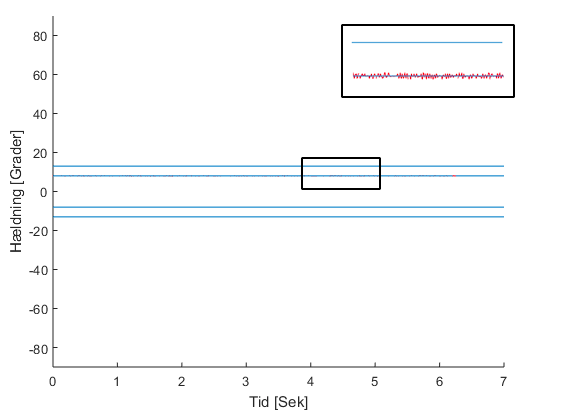
\includegraphics[width=0.51\textwidth]{figures/cProblemloesning/8Po.PNG}%
\hfill    
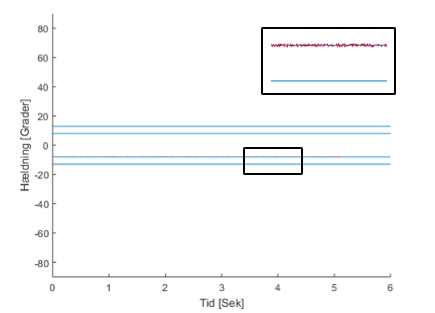
\includegraphics[width=0.51\textwidth]{figures/cProblemloesning/8Ne.PNG}%
}\\[0.3cm]% If you want some vertical space
\makebox[\textwidth]{%
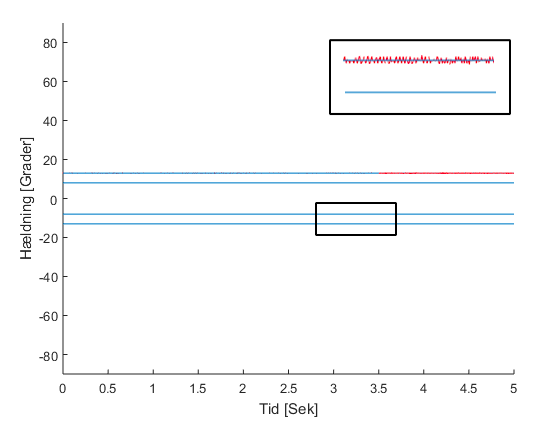
\includegraphics[width=0.51\textwidth]{figures/cProblemloesning/13Po.PNG}%
\hfill    
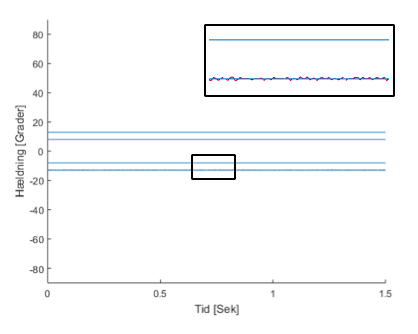
\includegraphics[width=0.51\textwidth]{figures/cProblemloesning/13Ne.PNG}%
}%
\caption{Figuren viser målingerne for de enkelte tærskelværdier. I følgende rækkefølge fra øvre venstre til nedre højre: $8^{\circ}$ positiv, $8^{\circ}$ negativ, $13^{\circ}$ positiv og $13^{\circ}$ negativ.}
\label{fig:software_grafer}
\end{figure}
\noindent Det fremgår af \figref{Fig:software_sinus}, at softwaren kan visualisere en hældning fra $\pm90^{\circ}$. Signalet opsamles og plottes realtime. Det vurderes, at softwaren kan anvendes til at visualisere kropshældning. 
\begin{figure}[H] 
	\centering 
	\includegraphics[scale=0.5]{figures/cProblemloesning/sinus.PNG}
	\caption{På figuren ses en sinuskurve, som illustrerer en svingning på $\pm$ $90^{\circ}$.}
	\label{Fig:software_sinus}
\end{figure}
\noindent På baggrund af testen vurderes det, at softwaren kan fremvise information om patientens hældning. Derudover visualiseres det, hvor hyppigt patienten har bevæget sig ud i risikozonerne via. referencelinjerne. Det er muligt at gemme data, som kan åbnes og analyseres. 